\begin{table*}[ht]
    \caption{Performance comparison of all baselines and our models. The best and second-best results are shown in bold and underlined, respectively. All values are multiplied by 100.}
    \centering
    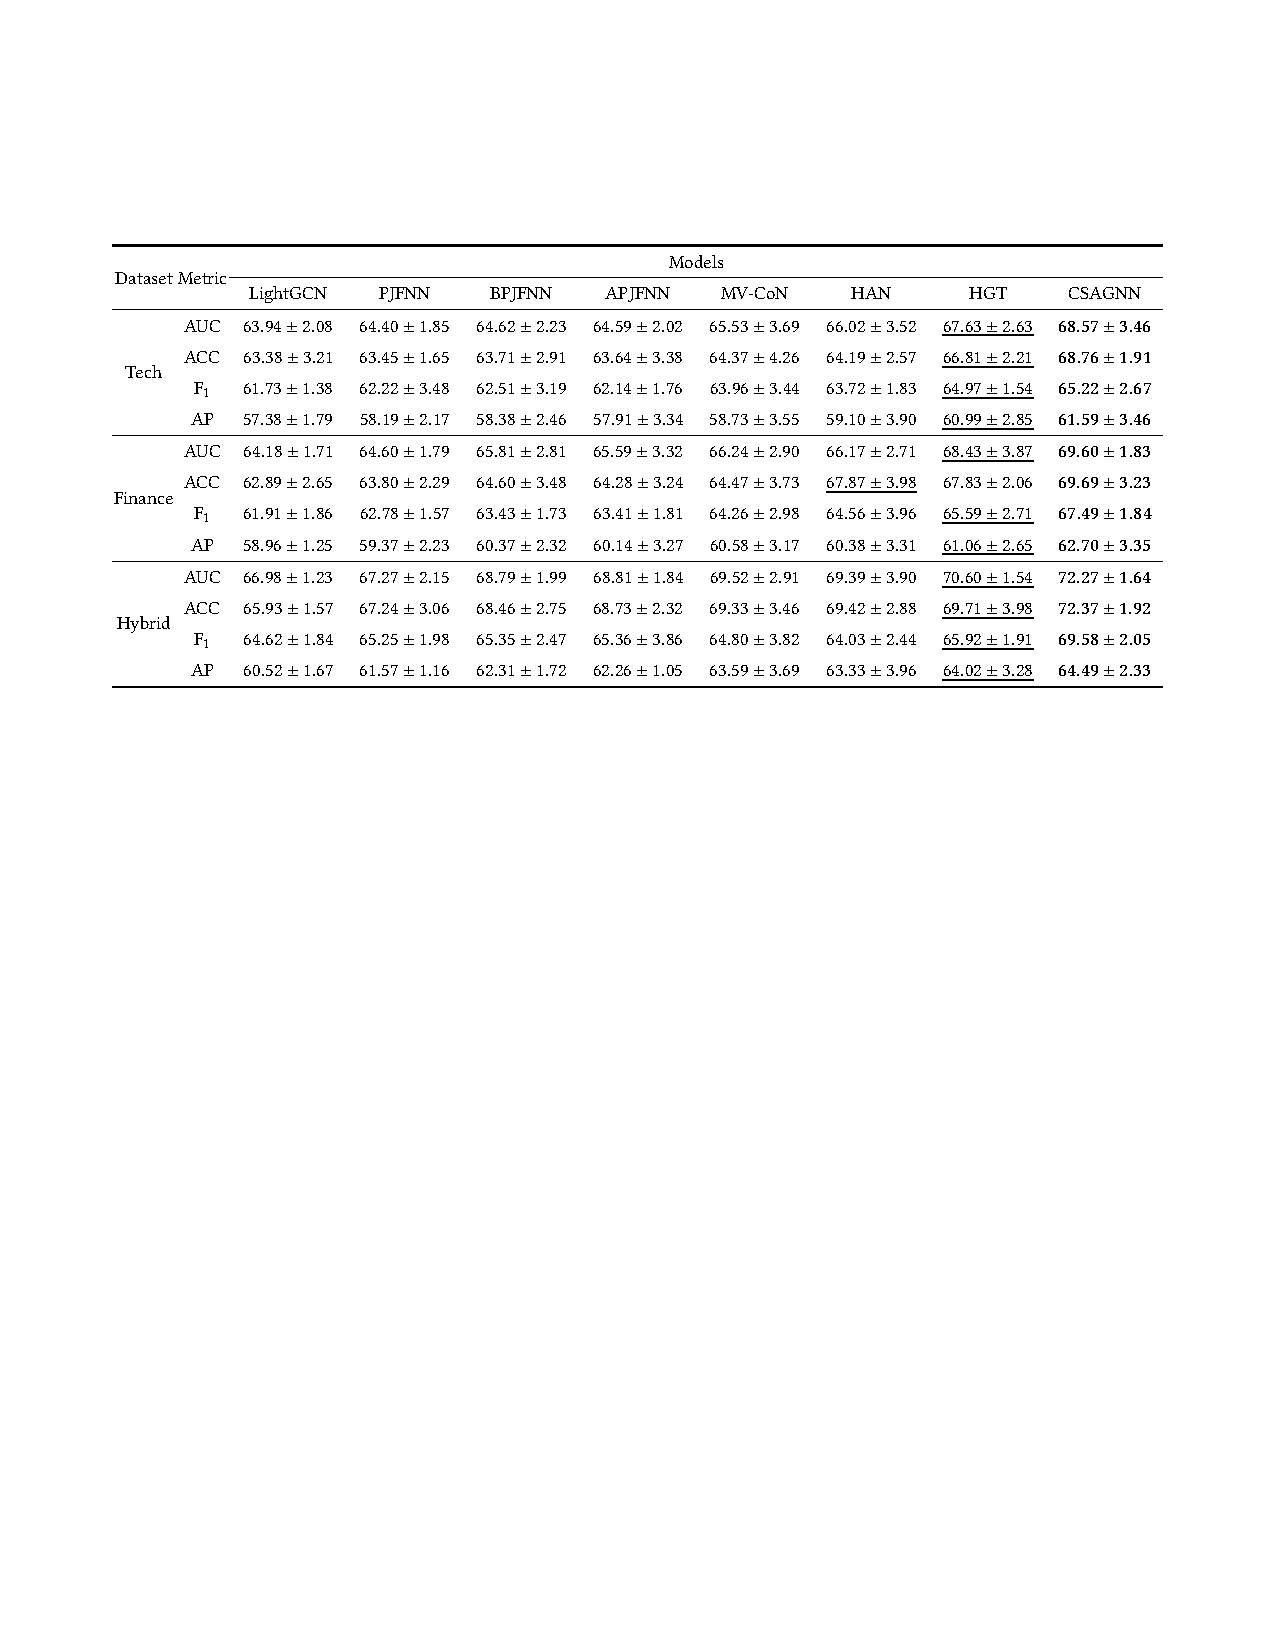
\includegraphics[width=.95\linewidth]{fig/results.pdf}
    \label{tab:Performance}
\end{table*}

\section{Experiments}

In this section, we will validate the performance of the CSAGNN model on three real datasets and answer the following research questions:

\begin{itemize}
    \item \textbf{RQ1}: Can CSAGNN outperform existing models on real-world datasets?
    \item \textbf{RQ2}: What are the effects of different components in our model?
    \item \textbf{RQ3}: Are professional networks helpful for the Person-Job Fit task?
    \item \textbf{RQ4}: Does the WHIN pre-training provide meaningful representations of skills for CSAGNN?
\end{itemize}

\subsection{Experiment Setup}

\subsubsection{Datasets}

We validate our model on three large real-world datasets from LinkedIn, a well-known workplace social platform. Datasets are divided by the industry to which the members and jobs belong. The first two datasets contain members and jobs from the technology and finance industries. Due to the singularity of the industry, social noise is limited. The third dataset, which includes members and jobs from various industries such as healthcare, education, and semiconductors, is intended to test the ability of CSAGNN to filter noise in professional networks. This hybrid dataset implies more complex social relationships and a wider range of job opportunities. The WHINs constructed from these three datasets all contain about 200,000 entities and 10 million links. Table \ref{tab:dataset statistic} displays the statistics of the datasets. The skills, schools, and companies in the dataset all come from explicit annotations by members or jobs on LinkedIn. We cannot provide further detailed information about the datasets to protect the users' privacy. Each candidate pair within the datasets is labeled as either positive or negative based on the feedback provided by members.

\begin{table}[ht]
  \caption{Statistics of datasets. M refers to Member, J refers to Job, S refers to Skill, CP refers to Candidate Pair, and PC refers to Professional Connection.}
  \label{tab:dataset statistic}
  \begin{tabular}{cccccc}
    \toprule
    \textbf{Industry} & \textbf{\#M} & \textbf{\#J} & \textbf{\#S} & \textbf{\#CP} &\textbf{\#PC}\\
    \midrule
    Tech        &       33000+   &       62000+ &  27000+ &   136000+  &   1922000+       \\
    Finance     &       20000+   &       27000+    & 23000+ & 36000+  &   615000+       \\
    Hybrid         &       83000+   &       120000+  & 33000+  &   200000+  &   2768000+       \\
    \bottomrule
  \end{tabular}
  % }
\end{table}


\subsubsection{Baseline Models}

We compare our model with the following baseline models.

\begin{itemize}
    \item \textbf{LightGCN \cite{he2020lightgcn}} is a simplified Graph Convolutional Network model for collaborative filtering with competitive performance and less complexity.
    \item \textbf{PJFNN \cite{zhu2018person}} is a method based on a convolutional neural network (CNN). Hierarchical CNN encodes Resumes and job descriptions independently, and the matching degree is calculated by cosine similarity.
    \item \textbf{BPJFNN \cite{qin2018enhancing}} leverages bidirectional LSTM to learn the representations of resumes and job descriptions. 
    \item \textbf{APJFNN \cite{qin2018enhancing}} leverages bidirectional LSTM and hierarchical attention mechanism to learn the representations of resumes and job descriptions.
    \item \textbf{MV-CoN \cite{bian2020learning}} combines text matching model and RGCN to learn representations of resumes and job descriptions.
    \item \textbf{HAN \cite{wang2019heterogeneous}} uses a dual attention mechanism to aggregate neighbor information via different metapaths.
    \item \textbf{HGT \cite{hu2020heterogeneous}} designs node- and edge-type dependent parameters to characterize the heterogeneous attention over each edge.
\end{itemize}



These baselines can be divided into three groups: (1) context-based models that treat Person-Job Fit as a text match problem and use contextual knowledge from members' profiles and jobs' descriptions: PJFNN, BPJFNN, APJFNN, and MV-CoN. In particular, MV-CoN additionally introduces structural information to enhance model performance. (2) collaborative filtering-based model that uses direct interactions between members and jobs: LightGCN. (3) end-to-end heterogeneous graph neural network models: HAN, HGT.

\subsubsection{Evaluation and Implementation Details}
We use four widely used metrics to evaluate the ranking performance: AUC, accuracy (ACC), F1, and average precision (AP).

The Person-Job Fit models, namely PJFNN, BPJFNN, and APJFNN, are implemented using RecBole—an established open-source recommendation library \cite{zhao2021recbole}. The MV-CoN model leverages the original code provided in their respective paper \cite{bian2020learning}. Other models are implemented with PyTorch Geometric \cite{Fey/Lenssen/2019}. We have employed BERT-Tiny\footnote{\url{https://huggingface.co/prajjwal1/bert-tiny}} to reduce computational costs.

The embedding dimensions for all models are standardized at 32. As discussed in Section \ref{link-level pre-training task}, subgraph sampling for mini-batch WHIN pre-training is executed using the PyTorch Geometric subgraph sampler \cite{Fey/Lenssen/2019}. Subgraph construction starts from nodes within a batch of candidate pairs, and each hop samples five neighbors via relations (or metapaths). Reconnecting all relations (and metapaths) between the sampled nodes follows this. We set the number of sampled hops to 3. The number of sampled hops is fixed at 3. In CSAGNN, the count of sampled skills ($n_s$) is designated as 10, and CSAGNN comprises two layers. The first 128 tokens from all text inputs are captured for all models. All models are optimized using the Adam optimizer \cite{kingma2014adam}, with a learning rate adjusted from 0.01 to 0.0001. For the purpose of evaluation, the dataset utilized across all models is randomly partitioned into a ratio of 8:1:1 for training, validation, and testing respectively. Three independent experiments are conducted, each one repeated, to ascertain consistent and reliable outcomes.

\subsection{The Overall Comparison (RQ1)}

Table \ref{tab:Performance} shows the performance of all baseline models and our model, CSAGNN. The results indicate better performance on the hybrid dataset than on individual industry datasets, possibly because jobs within the same industry are more similar and thus harder to distinguish. End-to-end heterogeneous graph neural network models have shown superior performance on all three datasets compared to context-based and CF-based models. HGT, utilizing heterogeneous knowledge, has improved AUC scores by 3.20\%, 3.31\%, and 1.55\% compared to the best baseline MV-CoN, which employs homogeneous knowledge. CSAGNN further improved AUC scores by 1.39\%, 1.71\%, and 2.37\% compared to HGT.

\begin{table}[ht]
    \caption{Ablation studies conducted on all datasets, with all values multiplied by 100.}
    \label{tab:ablation}
    \centering
    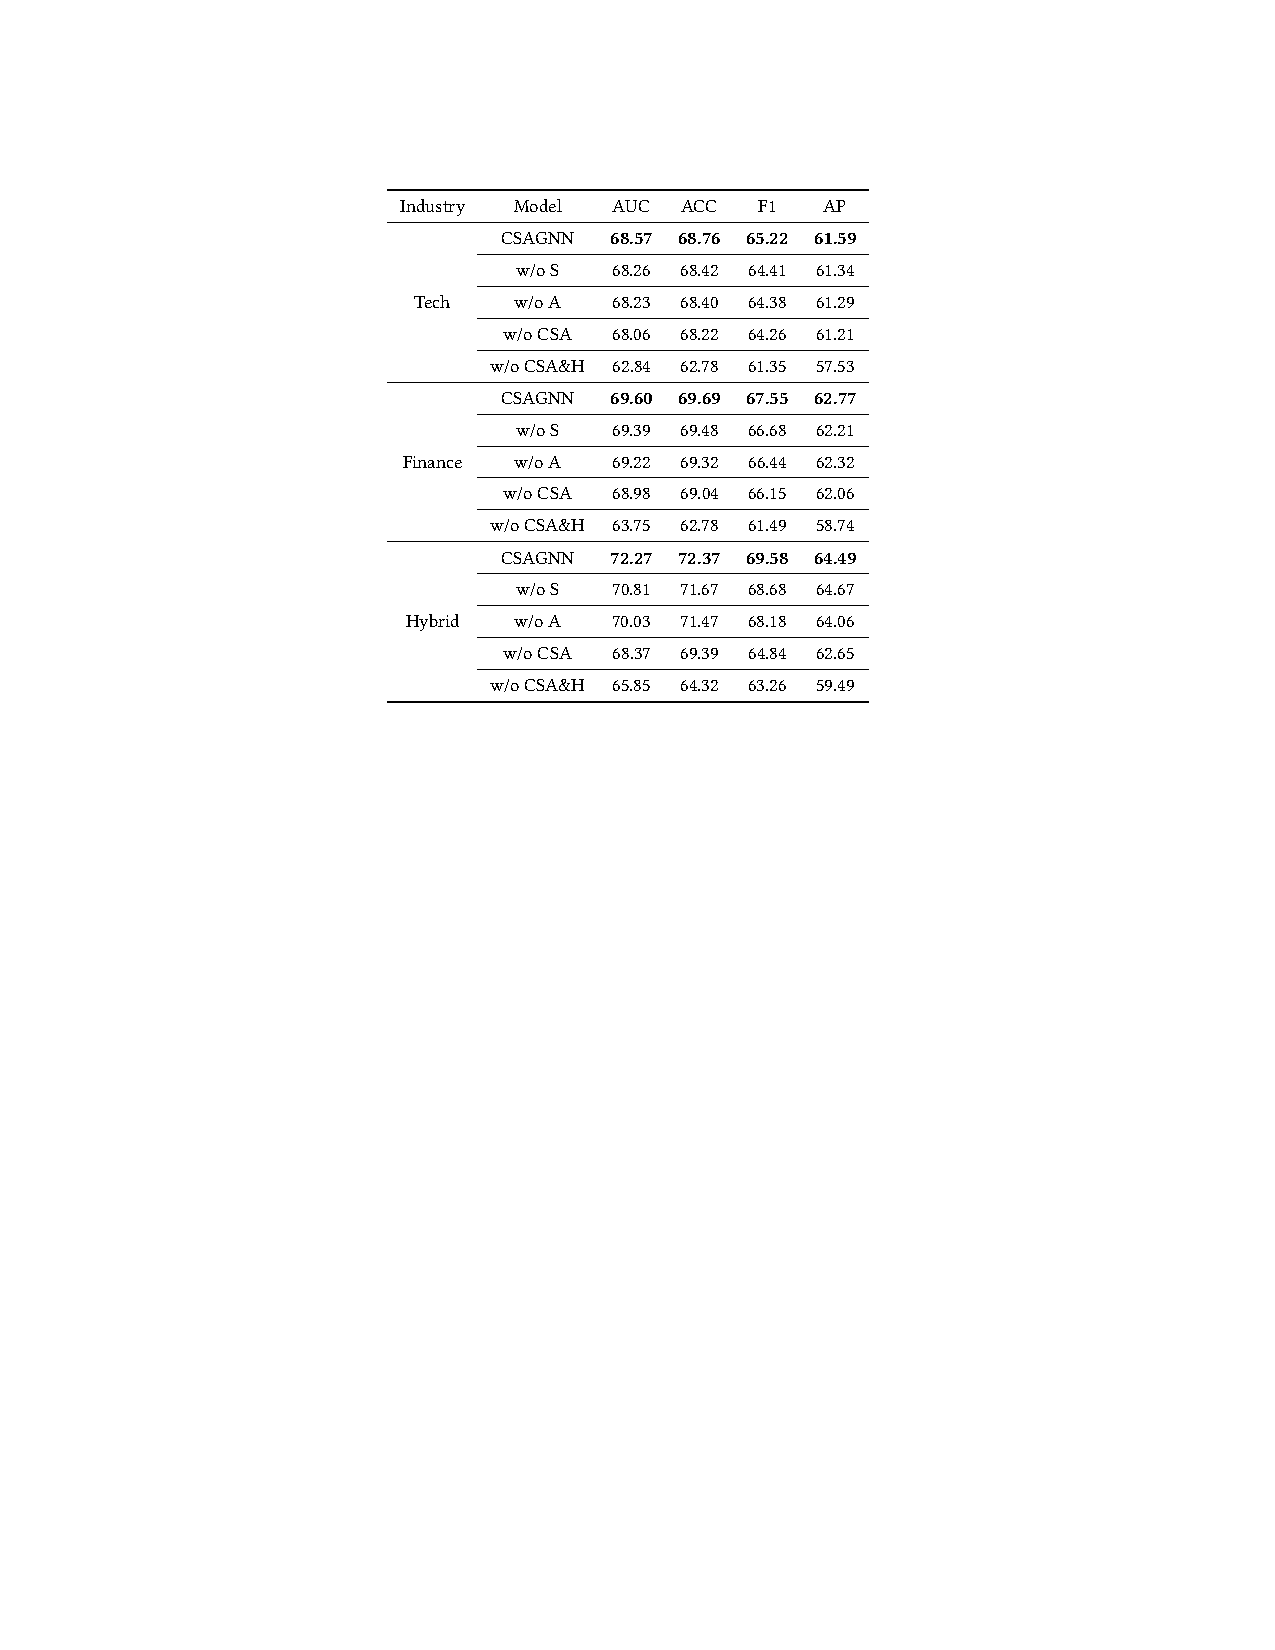
\includegraphics[width=0.95\linewidth]{fig/abalation.pdf}
\end{table}



\begin{figure}[ht]
    \centering
    \subfigure[Model performance varying the number of sampled skills while fixing CSAGNN layers to 1.]{
        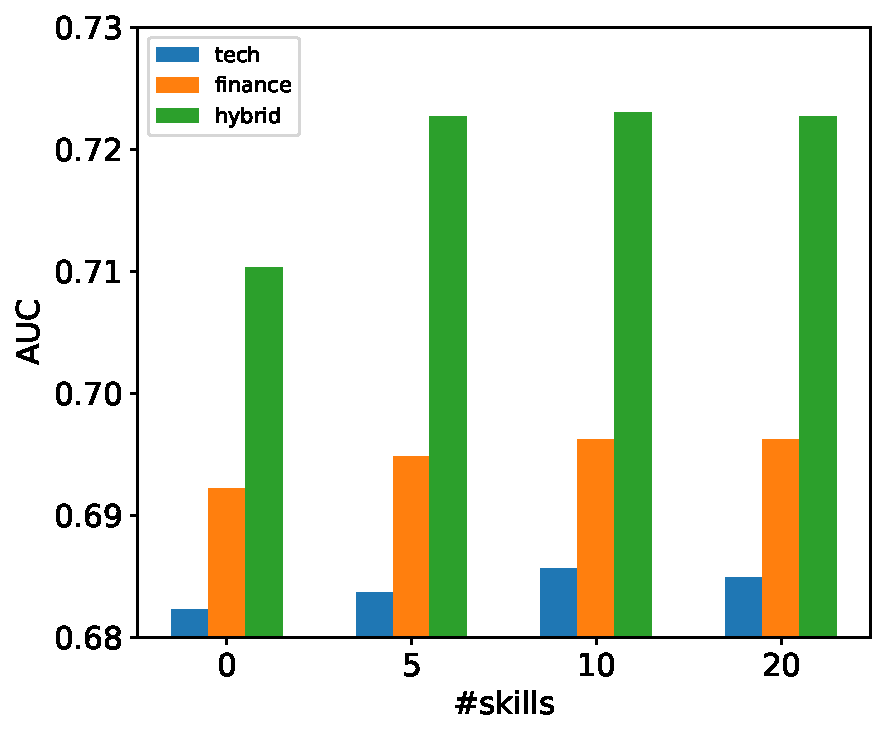
\includegraphics[width=.32\linewidth]{fig/skill_range.pdf}
        \hspace{0.2cm}
        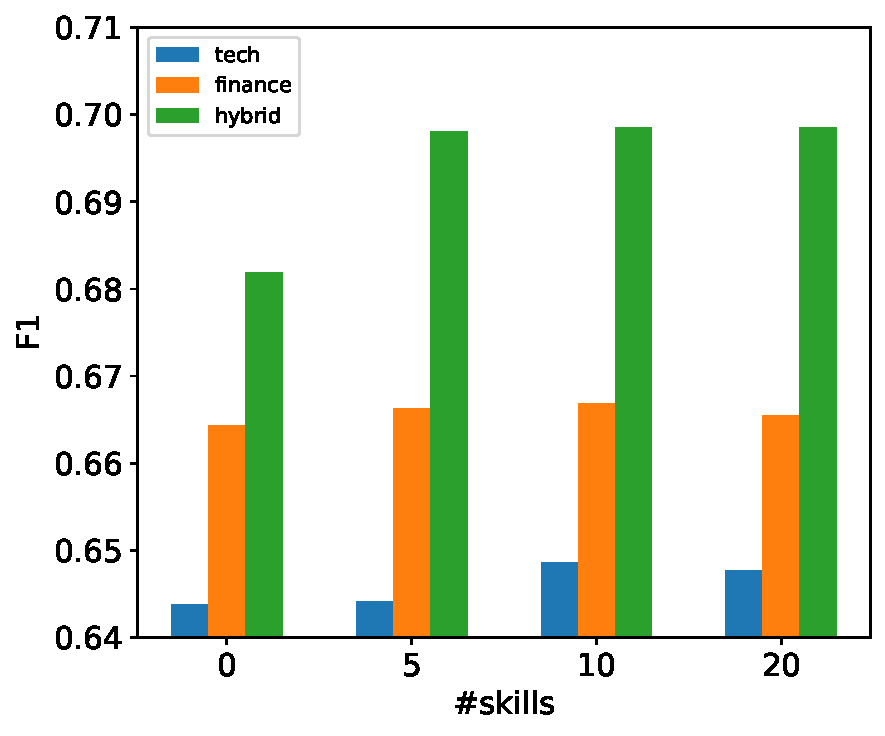
\includegraphics[width=.32\linewidth]{fig/skill_range_f1.pdf}
    }
    \\
    \subfigure[Model performance varying the number of CSAGNN layers while fixing the number of sampled skills to 10.]{
        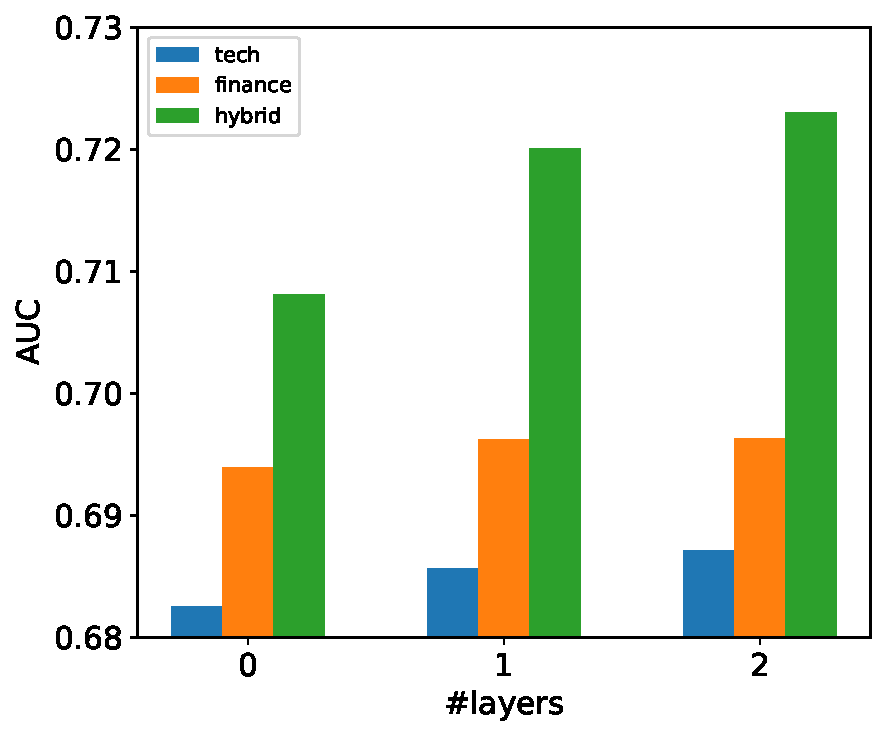
\includegraphics[width=.32\linewidth]{fig/hop_range.pdf}
        \hspace{0.2cm}
        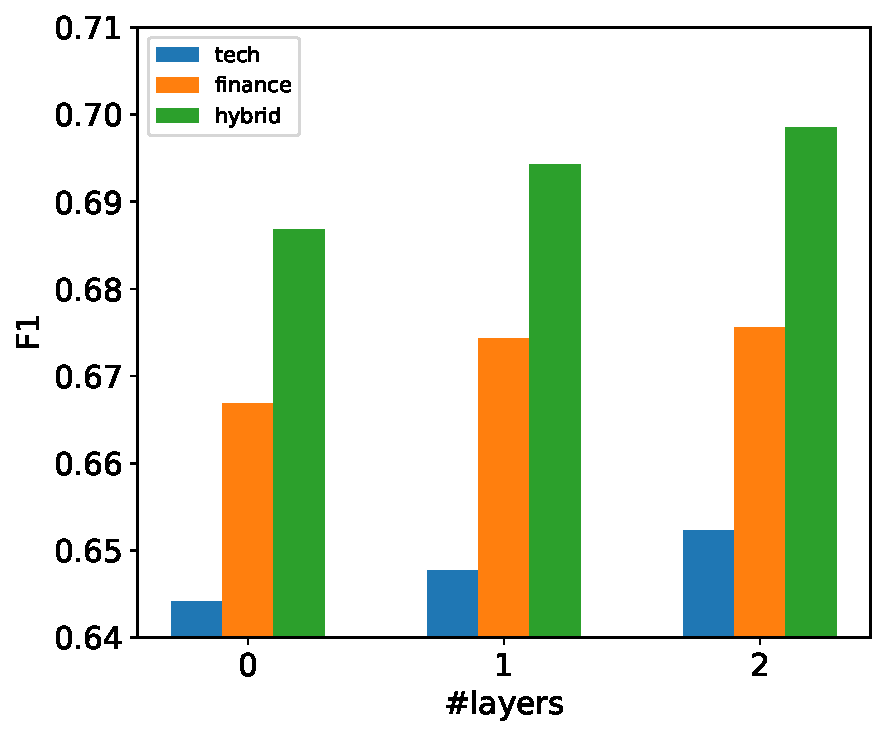
\includegraphics[width=.32\linewidth]{fig/hop_range_F1.pdf}
    }
    \caption{Hyperparameter tuning experiments to investigate the specific effects of social relations and job-specific attention mechanism.}
    \label{fig:skill_range}    
\end{figure}

\subsection{Ablation Studies and  Parameter Tuning (RQ2)}
\label{RQ2: Ablation Study}
Our approach employs two main techniques: WHIN pre-training, which integrates heterogeneous knowledge, including professional networks, and CSAGNN, which incorporates professional networks with an attention mechanism. We conducted ablation studies to analyze the effectiveness of different techniques, where we considered the following variants of CSAGNN: (1) CSAGNN w/o S removes messages from professional connections but retains the job-specific attention mechanism for members themselves. (2) CSAGNN w/o A removes the job-specific attention mechanism. (3) CSAGNN w/o CSA removes both professional connections and job-specific attention mechanisms, using only structural knowledge from the WHIN pre-train approach. (4) CSAGNN w/o CSA\&H removes WHIN pre-trained embeddings and CSA mechanism, only using text information as input and leverages MLP to predict.



\begin{figure*}[ht]
    \centering
    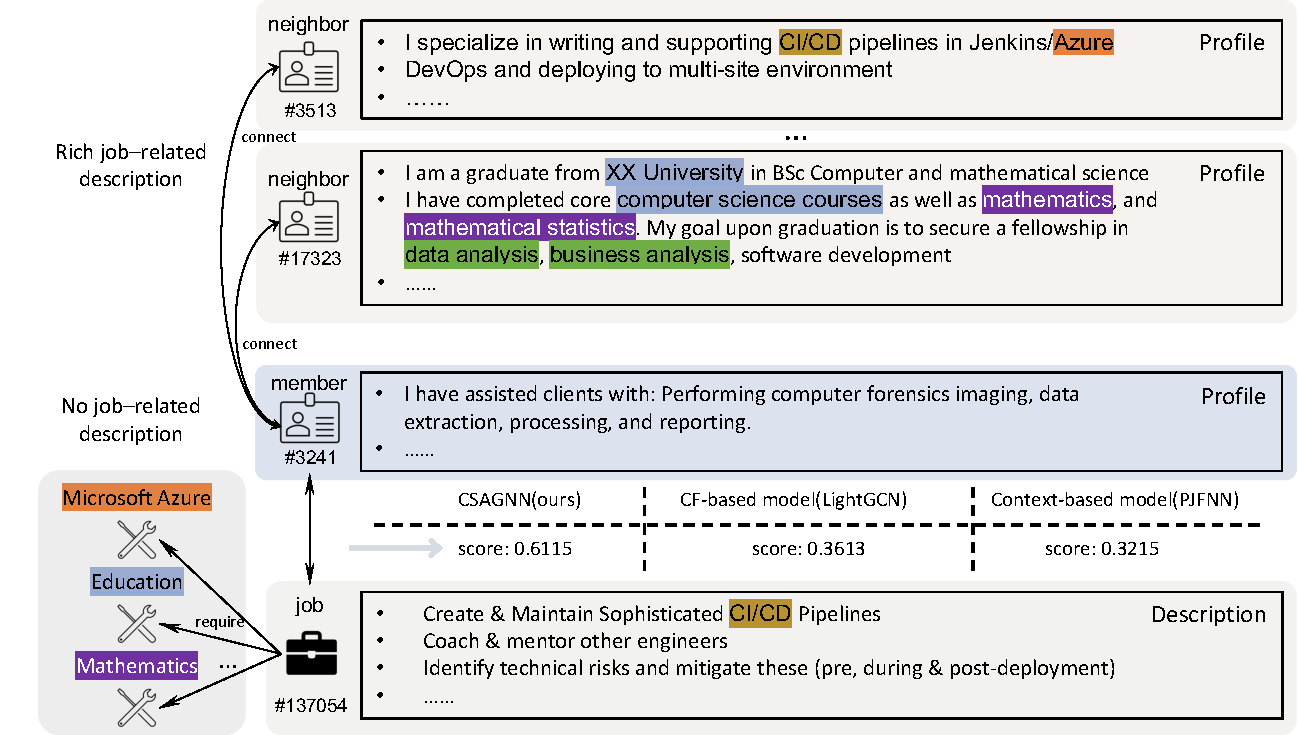
\includegraphics[width=0.53\textwidth]{fig/case_study.pdf}
    \caption{A case where professional connections improve performance on Person-Job Fit. CSAGNN can improve the performance of Person Job Fit by filtering and aggregating information from professional networks. For privacy protection reasons, we have rewritten the statement in the example while ensuring that the semantic information remains unchanged.}
    \label{fig:case}
\end{figure*}

\begin{figure}[ht]
    \centering
    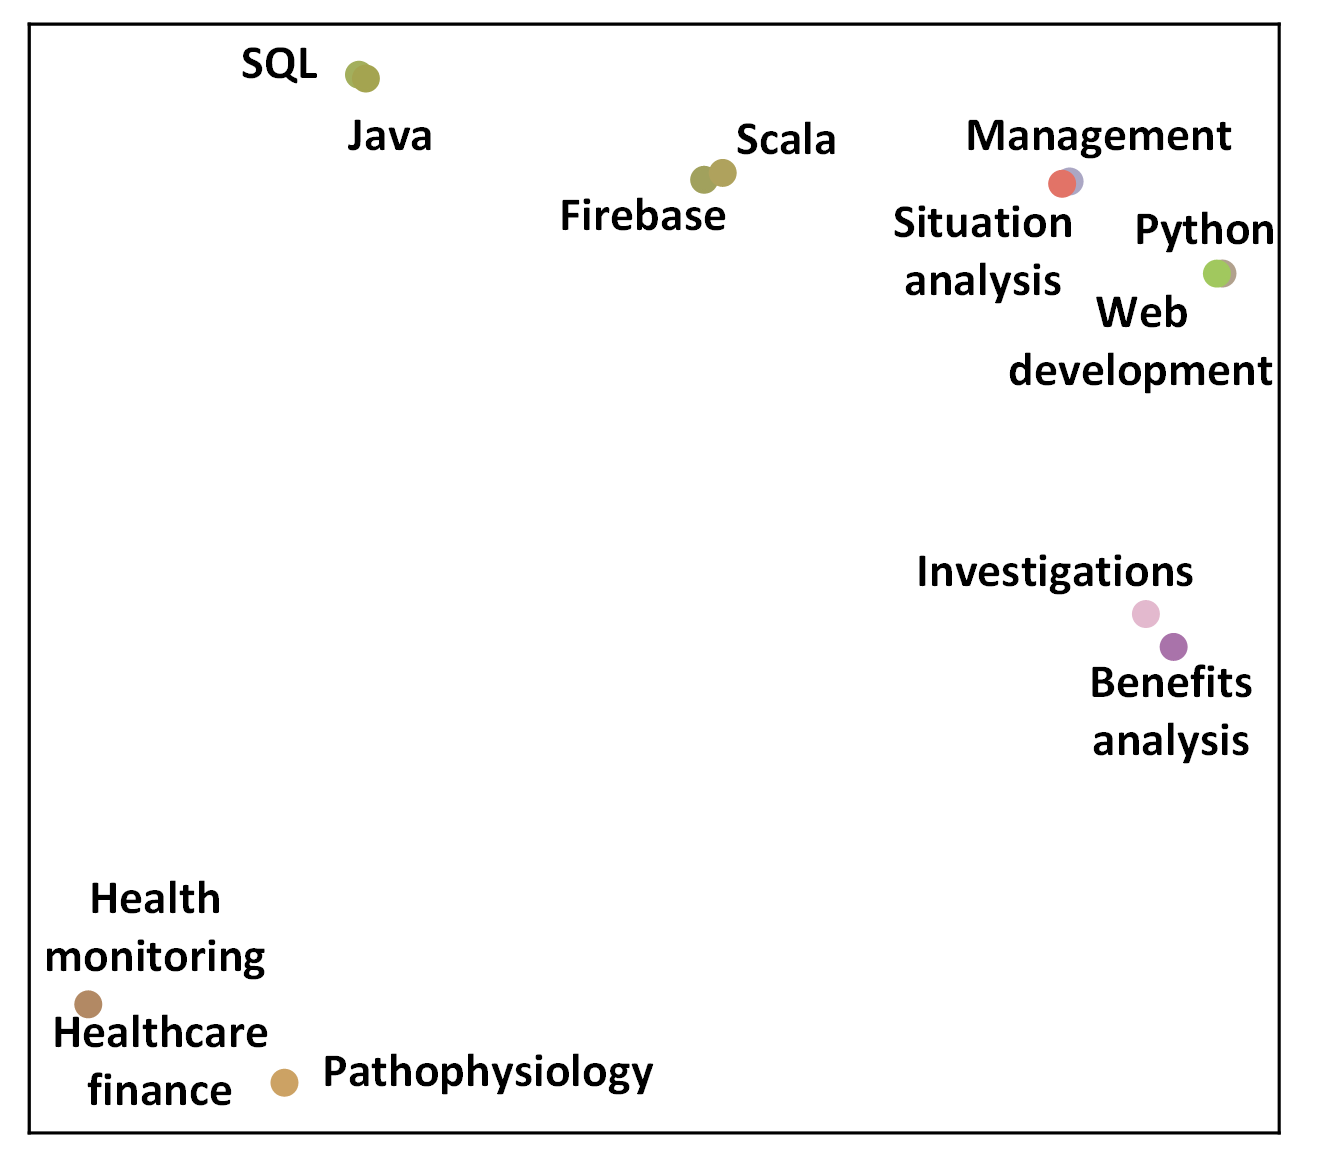
\includegraphics[width=.45\linewidth]{fig/skill_group.png}
    \caption{Visualization of WHIN Pre-trained skill embeddings showing clear distinction between Technology and Health-Related Skills.}
    \label{fig:skill_group}
\end{figure}



As detailed in Table \ref{tab:ablation}, within single industry datasets with low social noise, the job-specific attention mechanism and professional connections' messages yielded limited benefits. However, WHIN pre-training embeddings were crucial for enhancing performance. On hybrid datasets with high social noise, where candidate pairs may span different industries, the job-specific attention mechanism, along with the WHIN pre-training embedding, significantly improved the model.

To investigate the specific roles of professional networks and job-specific attention mechanisms in our model, we performed hyperparameter tuning experiments by fixing one module and varying the other to observe its impact on performance. Specifically, we first fixed the number of CSAGNN layers to 1 and tested the model's performance with different numbers of sampled skills ($n_s$), as described in Section \ref{Contextual Social Attention Graph Neural Network}. We then fixed $n_s$ to 10 and tested the model with different numbers of CSAGNN layers. The results on all datasets showed that, compared to the neighbor sampling range, the gain in model performance from the attention mechanism saturates when the number of sampled skills is relatively small. This observation led us to explore the balance between model performance and efficiency by selecting a smaller value for $n_s$.

\subsection{Case Study (RQ3)}
The value of utilizing professional networks is illustrated in the example shown in Figure \ref{fig:case}. In this case, we have rephrased the information to preserve the users' privacy while retaining its essential meaning. Even though the member's profile contains minimal information, the CSAGNN model adeptly predicts their classification by harnessing job-related insights from the member's professional connections. This contrasts sharply with the incorrect predictions made by the collaborative filtering-based LightGCN and context-based PJFNN models. This specific example accentuates the vital role of professional connections in the classification process and underlines the CSAGNN model's distinctive capability to leverage such relationships for precise predictions.


\subsection{Visualization (RQ4)}
To demonstrate the effectiveness of WHIN pre-training in capturing meaningful skill representations for CSAGNN, we analyzed the pre-trained embeddings of selected skills in the embedding space. Utilizing Principal Component Analysis (PCA) as our method of dimensional reduction \cite{jolliffe2016principal}, we were able to visualize the WHIN pre-trained embeddings for various skills. Figure \ref{fig:skill_group} reveals that skills closely related to programming, such as C++ and Python, are grouped together in the embedding space. In contrast, skills associated with healthcare form a distinct cluster. It is noteworthy that these classifications were achieved using only the skill names as initialization. Yet, our WHIN pre-training method successfully distinguishes between skill categories by learning from heterogeneous knowledge, highlighting the capability of WHIN to recognize and differentiate skills across multiple domains.
